\documentclass[aspectratio=169]{../latex_main/tntbeamer}  % you can pass all options of the beamer class, e.g., 'handout' or 'aspectratio=43'
\usepackage{dsfont}
\usepackage{bm}
\usepackage[english]{babel}
\usepackage[T1]{fontenc}
%\usepackage[utf8]{inputenc}
\usepackage{graphicx}
\graphicspath{ {./figures/} }
\usepackage{algorithm}
\usepackage[ruled,vlined,algo2e,linesnumbered]{algorithm2e}
\usepackage{hyperref}
\usepackage{booktabs}
\usepackage{mathtools}

\usepackage{amsmath,amssymb}

\DeclareMathOperator*{\argmax}{arg\,max}
\DeclareMathOperator*{\argmin}{arg\,min}

\usepackage{amsbsy}
\newcommand{\vect}[1]{\bm{#1}}
%\newcommand{\vect}[1]{\boldsymbol{#1}}

\usepackage{pgfplots}
\pgfplotsset{compat=1.16}
\usepackage{tikz}
\usetikzlibrary{trees} 
\usetikzlibrary{shapes.geometric}
\usetikzlibrary{positioning,shapes,shadows,arrows,calc,mindmap}
\usetikzlibrary{positioning,fadings,through}
\usetikzlibrary{decorations.pathreplacing}
\usetikzlibrary{intersections}
\pgfdeclarelayer{background}
\pgfdeclarelayer{foreground}
\pgfsetlayers{background,main,foreground}
\tikzstyle{activity}=[rectangle, draw=black, rounded corners, text centered, text width=8em]
\tikzstyle{data}=[rectangle, draw=black, text centered, text width=8em]
\tikzstyle{myarrow}=[->, thick, draw=black]

% Define the layers to draw the diagram
\pgfdeclarelayer{background}
\pgfdeclarelayer{foreground}
\pgfsetlayers{background,main,foreground}

% Requires XeLaTeX or LuaLaTeX
%\usepackage{unicode-math}

\usepackage{fontspec}
%\setsansfont{Arial}
\setsansfont{RotisSansSerifStd}[ 
Path=../latex_main/fonts/,
Extension = .otf,
UprightFont = *-Regular,  % or *-Light
BoldFont = *-ExtraBold,  % or *-Bold
ItalicFont = *-Italic
]
\setmonofont{Cascadia Mono}[
Scale=0.8
]

\renewcommand{\ttdefault}{Cascadia Mono}

% scale factor adapted; mathrm font added (Benjamin Spitschan @TNT, 2021-06-01)
%\setmathfont[Scale=1.05]{Libertinus Math}
%\setmathrm[Scale=1.05]{Libertinus Math}

% other available math fonts are (not exhaustive)
% Latin Modern Math
% XITS Math
% Libertinus Math
% Asana Math
% Fira Math
% TeX Gyre Pagella Math
% TeX Gyre Bonum Math
% TeX Gyre Schola Math
% TeX Gyre Termes Math

% Literature References
\newcommand{\lit}[2]{\href{#2}{\footnotesize\color{black!60}[#1]}}

%%% Beamer Customization
%----------------------------------------------------------------------
% (Don't) Show sections in frame header. Options: 'sections', 'sections light', empty
\setbeamertemplate{headline}{empty}

% Add header logo for normal frames
\setheaderimage{
	% 
\includegraphics[height=\logoheight]{figures/TNT_darkv4.pdf}
	
\includegraphics[height=\logoheight]{../latex_main/figures/Leibniz-AI-Academy_Logo}
	% 
\includegraphics[height=\logoheight]{figures/logo_tntluh.pdf}
}

% Header logo for title page
\settitleheaderimage{
	% 
\includegraphics[height=\logoheight]{figures/TNT_darkv4.pdf}
	
\includegraphics[height=\logoheight]{../latex_main/figures/Leibniz-AI-Academy_Logo}
	% 
\includegraphics[height=\logoheight]{figures/logo_tntluh.pdf}
}

% Title page: tntdefault 
\setbeamertemplate{title page}[tntdefault]  % or luhstyle
% Add optional title image here
%\addtitlepageimagedefault{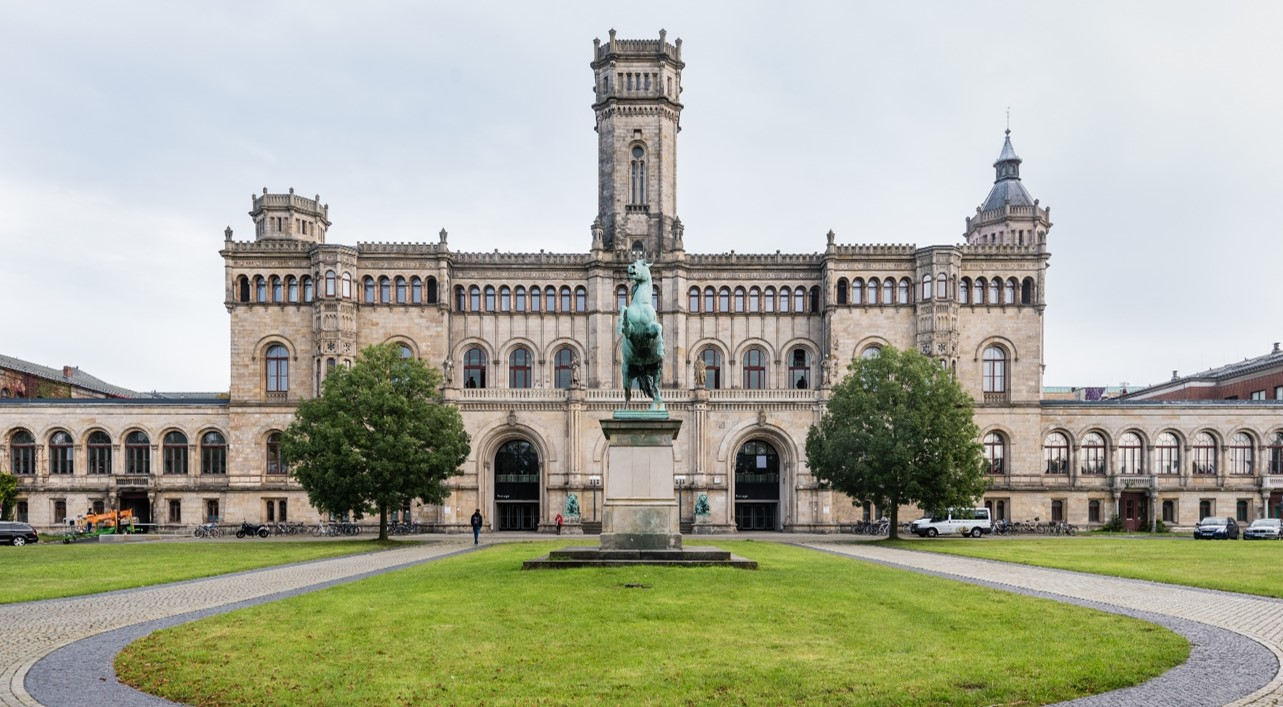
\includegraphics[width=0.65\textwidth]{figures/luh_default_presentation_title_image.jpg}}

% Title page: luhstyle
% \setbeamertemplate{title page}[luhstyle]
% % Add optional title image here
% \addtitlepageimage{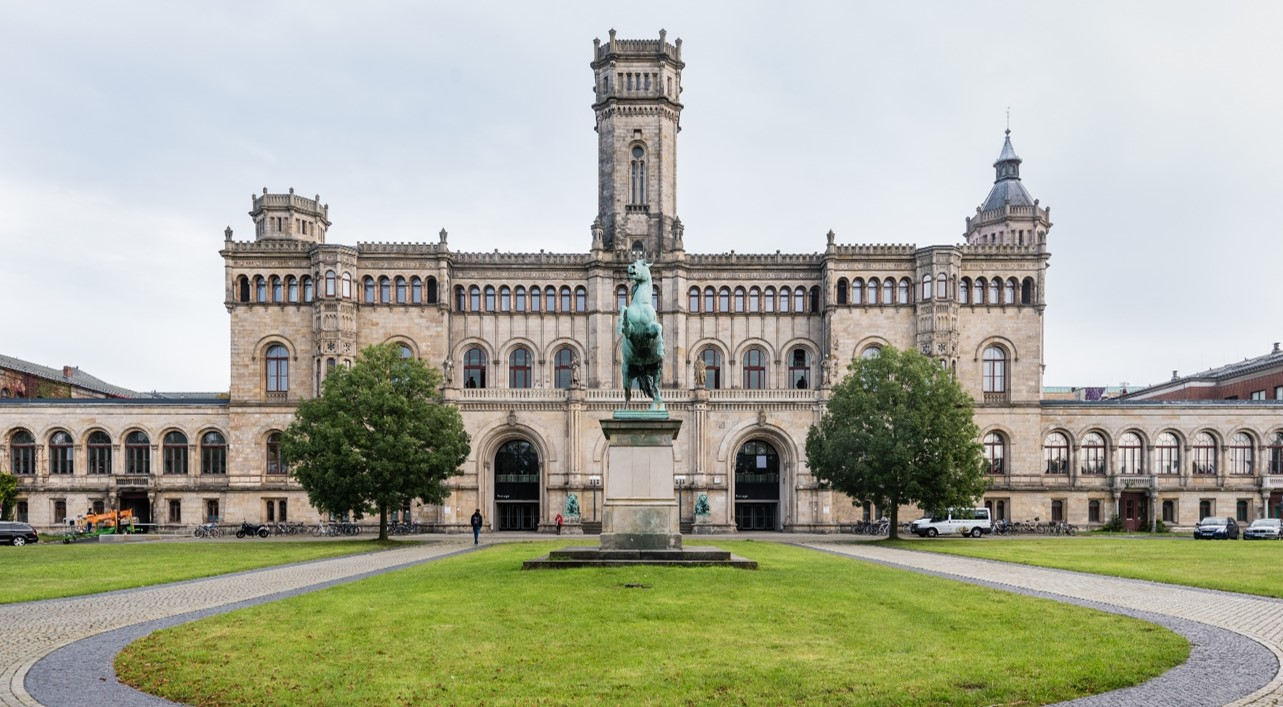
\includegraphics[width=0.75\textwidth]{figures/luh_default_presentation_title_image.jpg}}

\author[Abedjan \& Lindauer]{Ziawasch Abedjan \& \underline{Marius Lindauer}\\[1em]
	%
\includegraphics[height=\logoheight]{../latex_main/figures/luh_logo_rgb_0_80_155.pdf}\qquad
	
\includegraphics[height=\logoheight]{../latex_main/figures/DBIS_Kurzlogo.png}\qquad
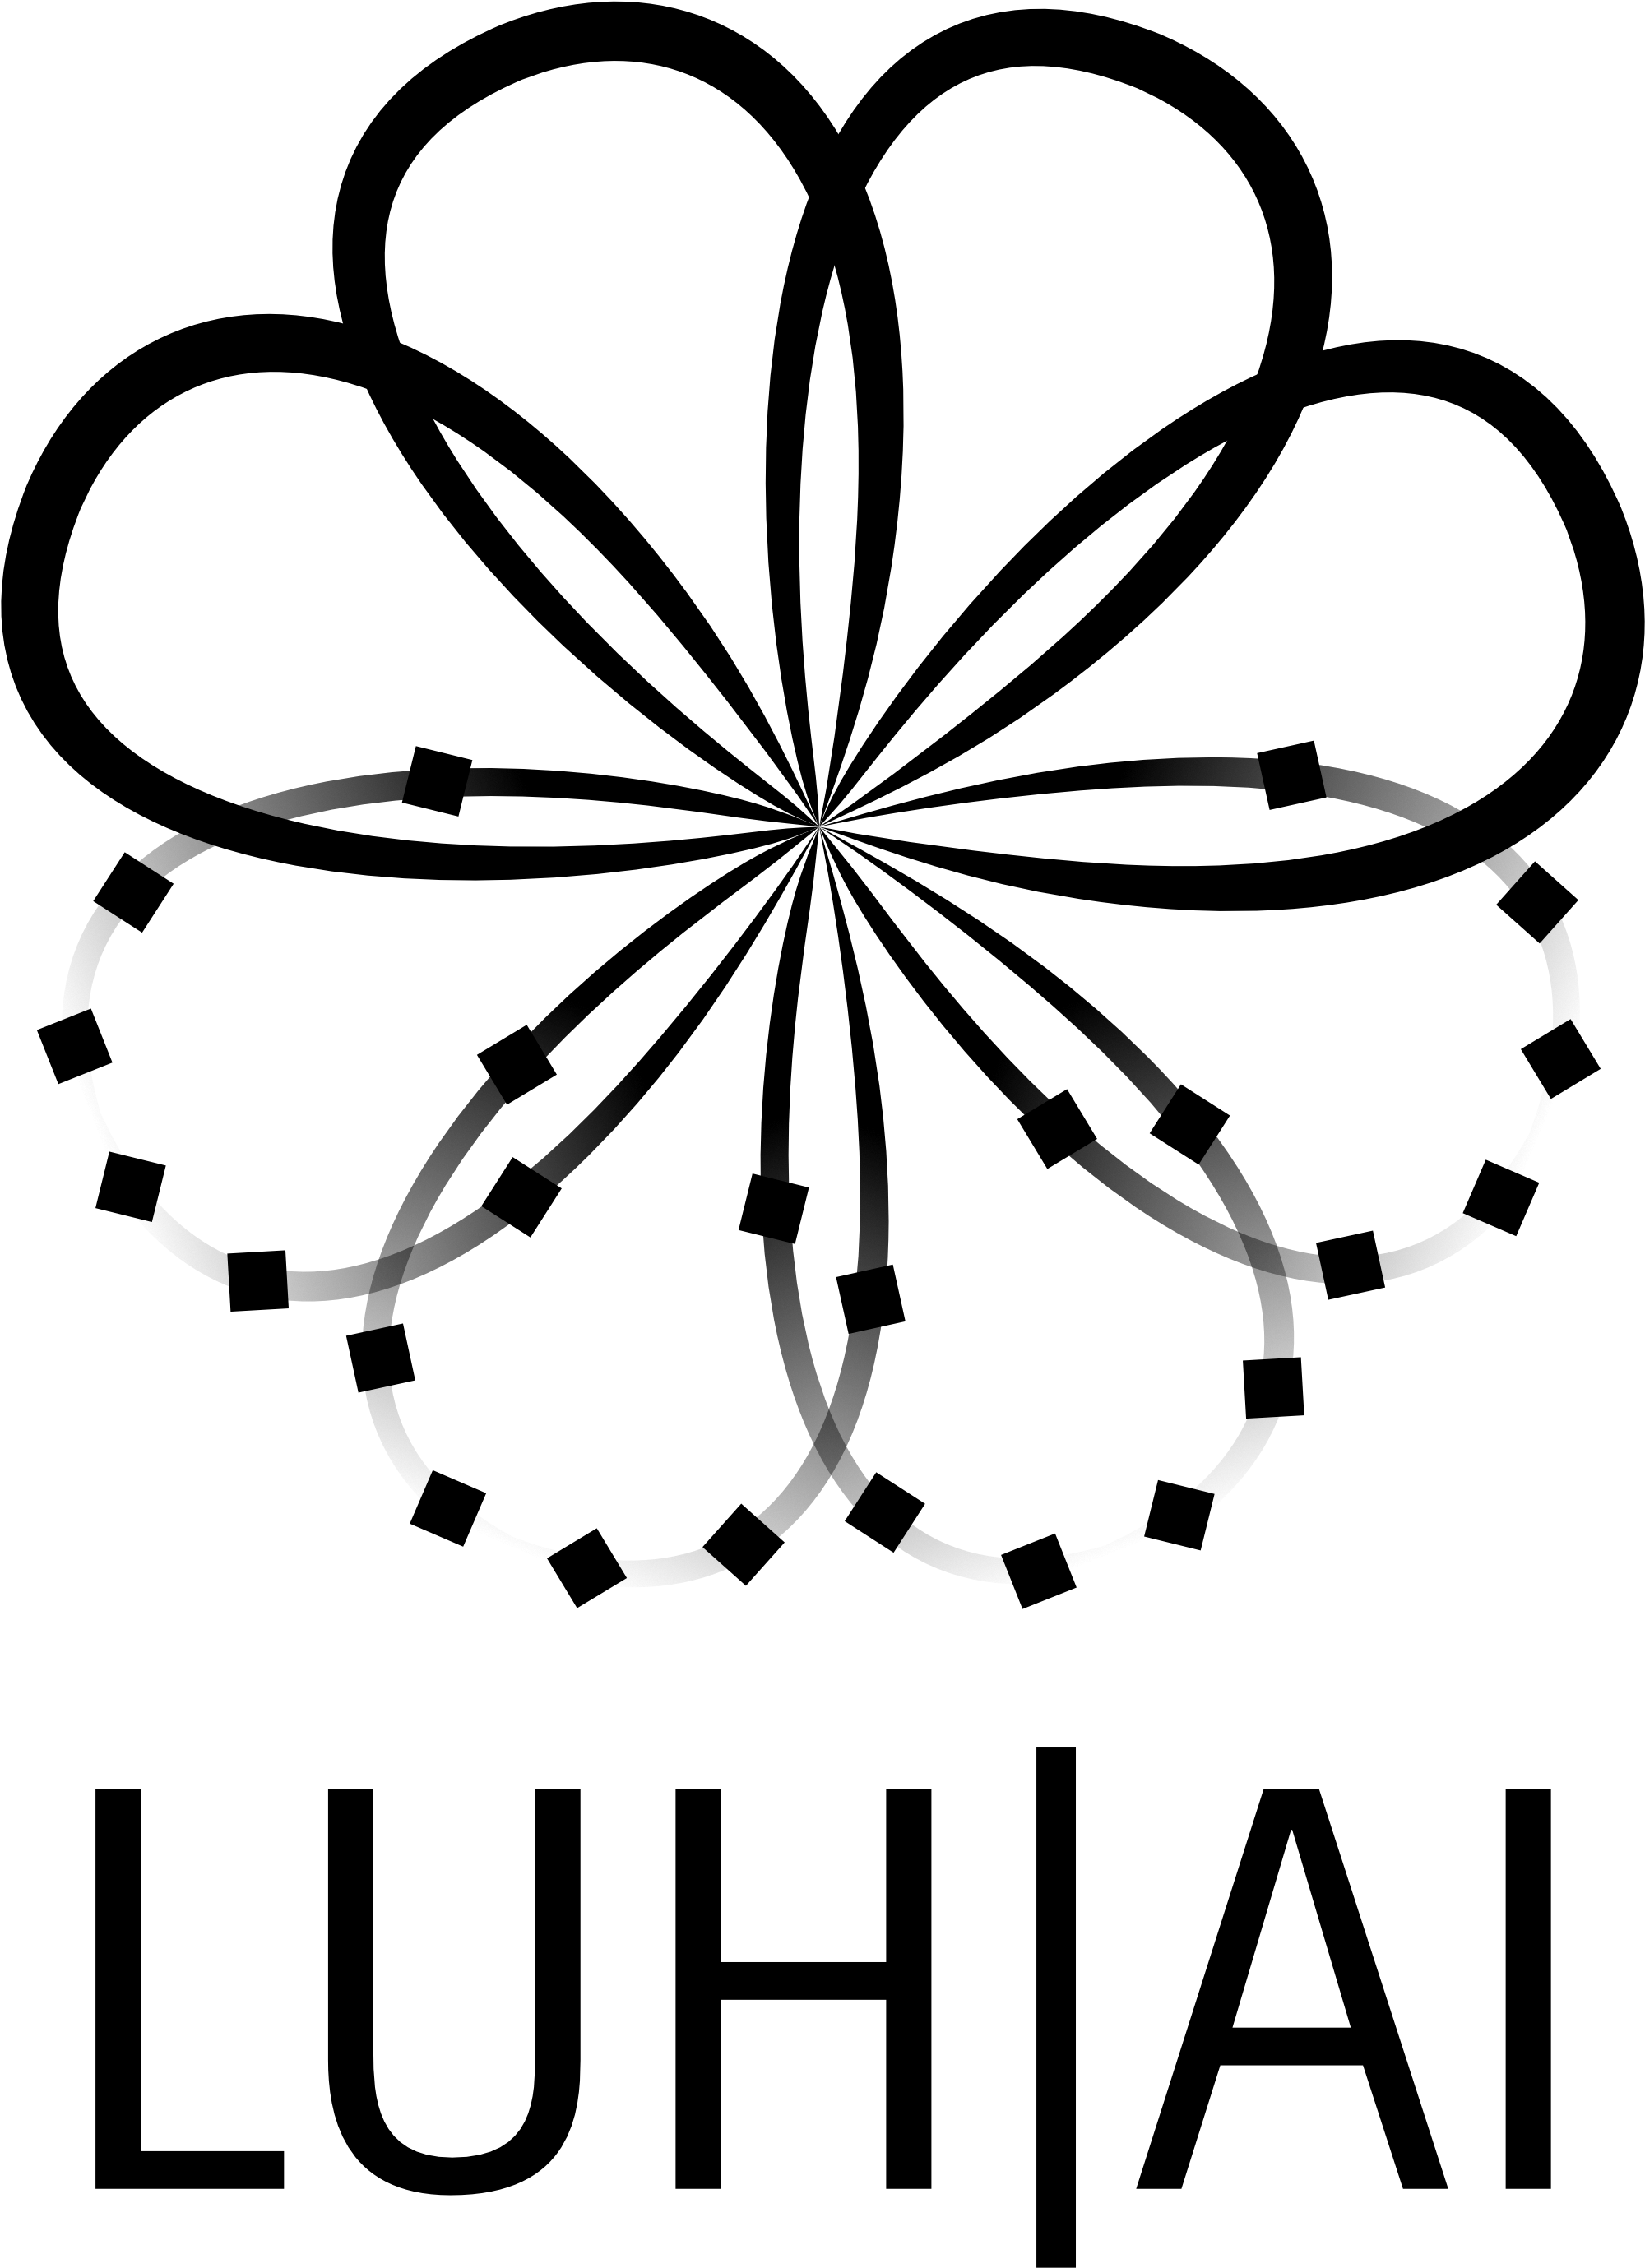
\includegraphics[height=\logoheight]{../latex_main/figures/logo_short_highres_black}\qquad

\includegraphics[height=\logoheight]{../latex_main/figures/Leibniz-AI-Academy_Logo}\qquad
%
\includegraphics[height=\logoheight]{../latex_main/figures/L3S.jpg}	
}
\date{\hspace{0.5em} {
\includegraphics[height=1.5em]{../latex_main/figures/Cc-by-nc-sa_icon.svg.png}}; extension of \href{https://ds100.org/fa21/}{[DS100]}
}


%%% Custom Packages
%----------------------------------------------------------------------
% Create dummy content
\usepackage{blindtext}

% Adds a frame with the current page layout. Just call \layout inside of a frame.
\usepackage{layout}


%%% Macros
%\renewcommand{\vec}[1]{\mathbf{#1}}
% \usepackage{bm}
%\let\vecb\bm

\title[Cross Entropy Loss]{DS: Classification}
\subtitle{Cross Entropy Loss}

\graphicspath{ {./figure/} }
%\institute{}


\begin{document}
	
	\maketitle
	\begin{frame}{Log loss}
	    \begin{columns}
	        \begin{column}{.5\textwidth}
	                Consider this new loss, called the (negative) log loss, for a single observation\\ \alert{when the true $y$ is equal to $1$.}\\
	                \bigskip
	                We can see that as our prediction gets further and further from 1, the loss approaches infinity (unlike squared loss, which maxed out at 1).
	        \end{column}
	        
	        \begin{column}{.4\textwidth}
	                    
	                    \centering
	                    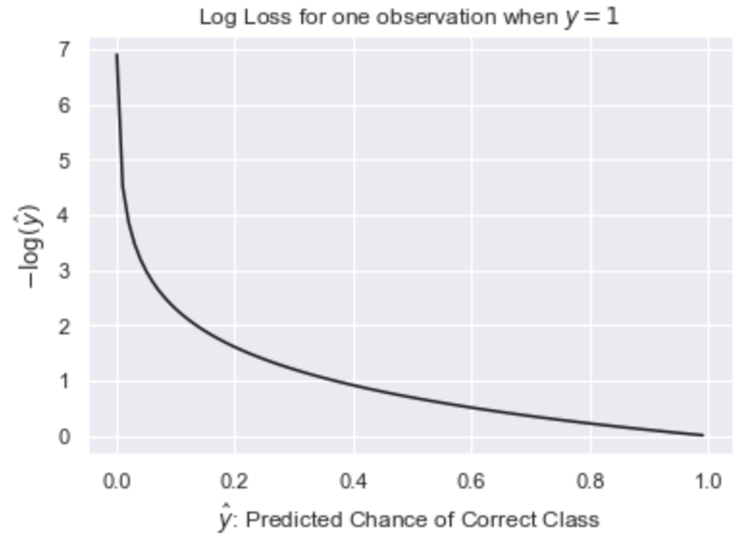
\includegraphics[scale=.5]{Bild18}
	        \end{column}
	    \end{columns}
	\end{frame}
	
	
	
% 	\begin{frame}{Log loss}
% 	    Let’s look at some losses in particular:
%         \begin{figure}
%             \centering
%             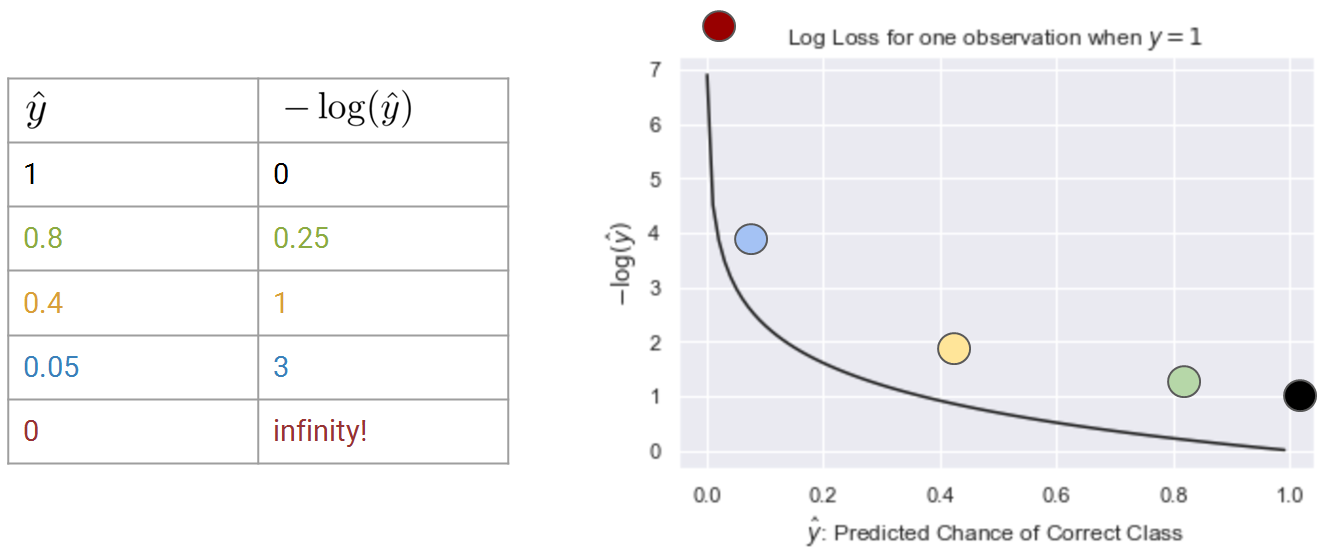
\includegraphics[scale=.33]{Bild19}
%         \end{figure}
% 	    Note: The logistic function never outputs 0 or 1 exactly, so there’s never a loss of  0 or infinite 
% 	\end{frame}
	
	\begin{frame}{Log loss}
	    So far, we’ve only looked at log loss when the correct class was 1. \\
	    What if our correct class is 0?
        \begin{figure}
            \centering
            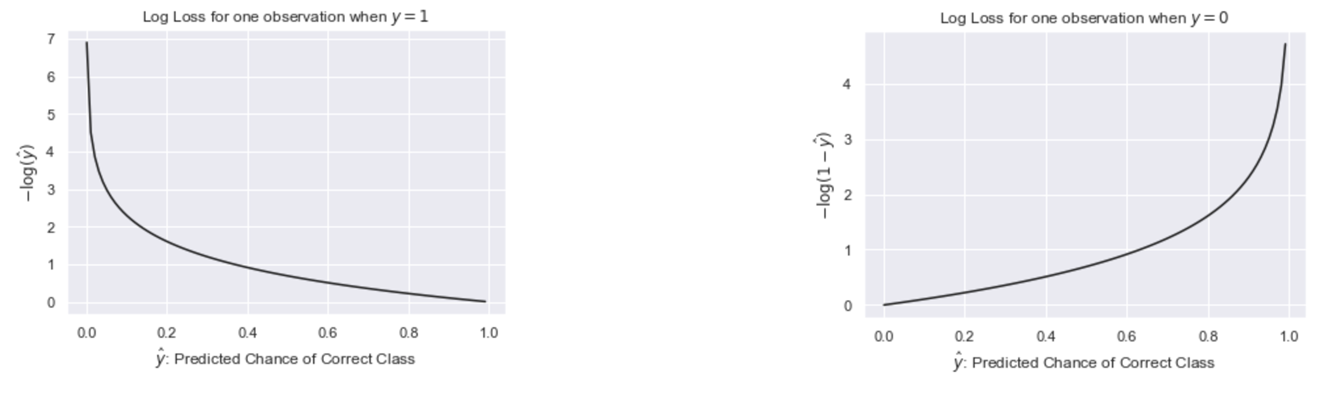
\includegraphics[scale=.33]{Bild20}
        \end{figure}
	    If the correct class is 0, we want to have low loss for values of   $\hat{y}$   close to 0, and high loss for values of   $\hat{y}$    close to 1. This is achieved by just “flipping” the plot on the left!
	\end{frame}
	
	
	\begin{frame}{Cross-entropy loss}
	    We can combine the two cases from the previous slide into a single loss function:
	    \begin{align*}
	        loss = \left\{\begin{array}{cc}
	            -log(1 - \hat{y}) & y = 0  \\
	            -log(\hat{y}) & y= 1 
	        \end{array}\right.
	    \end{align*}
	    This is often written unconditionally as:
	    \begin{equation*}
	        \text{loss} = -y\log (\hat{y}) - (1 - y) \log (1 - \hat{y})
	    \end{equation*}
	    Note: Since y = 0 or 1, one of these two terms is always equal to 0, which reduces this equation to the piecewise one above.\\
	    \bigskip
	    We call this loss function \alert{cross-entropy loss} (or “log loss”).
	\end{frame}
	
	\begin{frame}{Mean cross-entropy loss}
	    The empirical risk for the logistic regression model when using cross-entropy loss is then
	    \begin{align*}
	        R(\bm{\theta}) = -\frac{1}{n}\sum\limits_{i=1}^n(y_i\log (\underbrace{\sigma (\mathbb{X}_i^T\bm{\theta})}_{\hat{y}}) + (1 - y_i)\log (1 - \underbrace{\sigma (\mathbb{X}_i^T\bm{\theta})}_{\hat{y}}))
	    \end{align*}
	    Benefits over mean squared error for logistic regression:
	    \begin{itemize}
	        \item Loss surface is guaranteed to be convex.
	        \item More strongly penalizes bad predictions.
	        \item Has roots in probability and information theory.
	    \end{itemize}
	\end{frame}
	
	
	\begin{frame}{Comparing loss surfaces}
    
	        \centering
	        
	        Mean Squared Error (MSE) \hspace{2.5cm} Cross-Entropy Loss
	        
	        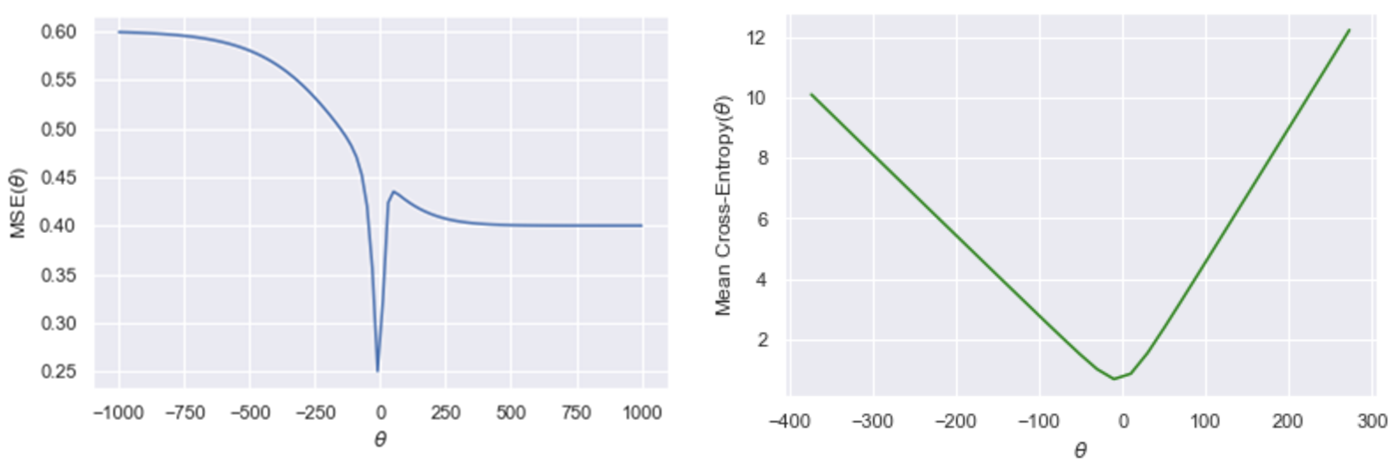
\includegraphics[scale=.35]{Bild21}
	\end{frame}
	
	
	\begin{frame}{Comparing loss surfaces}

	        \centering
	        
	        Mean Squared Error (MSE) \hspace{2.5cm} Cross-Entropy Loss
	        
	        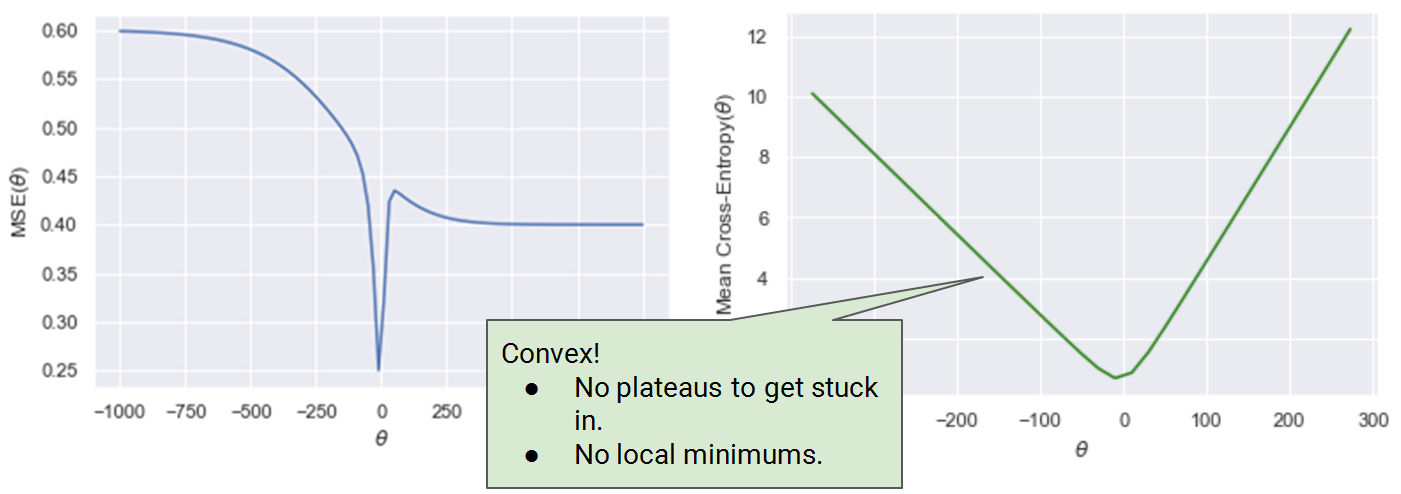
\includegraphics[scale=.35]{Bild22}
	\end{frame}
	
	
	\begin{frame}{Comparing loss surfaces}
	    \begin{figure}
	        \centering
	        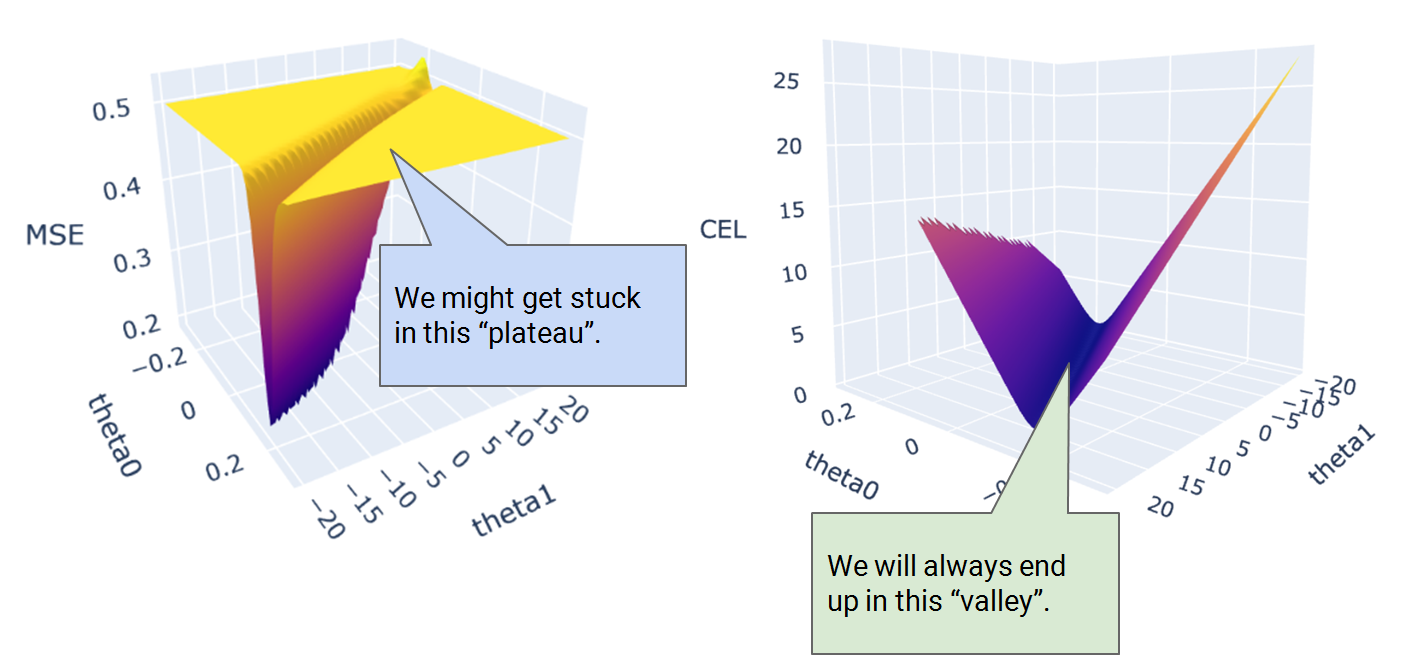
\includegraphics[scale=.35]{Bild23}
	    \end{figure}
	\end{frame}
	
	
	\begin{frame}[c]{Modeling recipe}
	    As per usual:
	    \begin{itemize}
	        \item[1]  Choose a model.
	        \item[2] Choose a loss (and, optionally, a regularization penalty).
	        \item[3] Minimize empirical risk for the given model, loss, and regularization penalty (using an analytical solution, or numerical technique like gradient descent).
	    \end{itemize}

	    \begin{itemize}
	        \item Using squared loss and using cross-entropy loss will usually result in different  $\hat{\bm{\theta}}$
	        \begin{itemize}
	            \item Different optimization problems, different solutions.
	            \item  Constant model: absolute loss meant median, squared loss meant mean.
	        \end{itemize}
	        \item Cross-entropy loss is often better than squared loss for logistic regression.
	        \begin{itemize}
	            \item Convex, so easier to minimize using numerical techniques
	            \item Better suited for modeling probabilities.
	        \end{itemize}
	    \end{itemize}
	\end{frame}
	
	\begin{frame}{Summary Logistic regression}
	    \begin{itemize}
	        \item In a logistic regression model, our goal is to predict a binary categorical variable\\ (Class 0 or Class 1) as a linear function of features, passed through the logistic function.
	        \begin{itemize}
	            \item Our response is the probability that our observation belongs to class 1.
	            \begin{equation*}
	                \hat{y} = f_{\bm{\theta}}(\bm{x}) = P(Y=1|\bm{x}) = \sigma (\bm{x}^\intercal\theta)
	            \end{equation*}
	            \item We arrived at this model by assuming that the log-odds of the probability of belonging to Class 1 is linear.
	            \item To find  $\hat{\bm{\theta}}$, we can choose squared loss or cross-entropy loss.
                \begin{itemize}
                    \item Squared loss works, but is often not a good idea.
                    \item Cross-entropy loss is much better (convex, better suited for modeling probabilities).
                \end{itemize}
	        \end{itemize}
	    \end{itemize}
	\end{frame}
	
\end{document}